
\documentclass[ 12pt, a4paper ]{article}

%packages
\usepackage{physics}
\usepackage{amsmath}
\usepackage{algorithm}
\usepackage{algorithmic}
\usepackage{graphicx}
\graphicspath{{../graphics/} }

\title{Ordinary least squares regression of Franke's function}
%\subtitle{subtitle here}

\author{Anders Eriksen}
\date{}

%//////////////////////
\begin{document}
%=====
%table of contents, list of figs and content
\maketitle
\tableofcontents
\listoffigures
\listoftables
%=====
\begin{abstract}
    The main summary of the work
\end{abstract}

\section{introduction}
    aims and rationale of the physics case, what you've done as well as a brief summary of 
the report \\
    o   Motivate the reader\\
    o   What done\\
    o   Structure of report\\
\section{Methods}
    Theoretical models and technicalities. \\
    o   describe methods and algorithms\\
    o   explain implementation of methods and say something about the structure of
        algorithm and present parts of code\\
    o   Plug in some calculations to test code, such as selected runs used to validate and
        verify results. Latter extremely important. Reader needs to know that your code
        reproduces selected benchmarks and reproduces previous results, either numerical 
        and/or well-known closed-form expressions. \\

The aim is to study regression models on data. These create a continuous function with which
the input data is fitted. The first, and most basic is the \textit{Ordinary Least Squares method} 
(\textit{OLS})

To test and validate the algorithms, a closed form function is an advantage. We wish to predict
terrain. there is a 2-dimensional function called \textit{Franke's function}\cite{} which can 
transform a set of coordinate vectors with values between $[0, 1]$ into height values through 
a sum of weighted exponents. 
\begin{align}
    f(x, y) \;=\; 
        &\frac{3}{4} \exp{ - \frac{(9x \,-\, 2)^2}{4}    \,-\, \frac{(9y \,-\, 2)^2}{4} }
    \nonumber \\
    +   &\frac{3}{4} \exp{ - \frac{(9x \,+\, 1)^2}{49}   \,-\, \frac{(9y \,+\, 1)  }{10} }
    \nonumber \\
    +   &\frac{1}{2} \exp{ - \frac{(9x \,-\, 7)^2}{4}    \,-\, \frac{(9y \,-\, 3)^2}{4} }
    \nonumber \\
    -   &\frac{1}{5} \exp{ -       (9x \,-\, 4)^2        \,-\,       (9y \,-\, 7)^2     }
    \label{eq:franke}
\end{align}

To generate the data, one can create a uniformly distributed set of initial values ordered 
from low to high. These initial arrays are then combined into coordinate data through the 
numpy meshgrid function before being passed to Franke's function. These are matrices, and 
they are therefore flattened to 1D arrays through numpy's \textit{ravel()} function.

Next comes setting up the model. Firstly, constructing the model design matrix. We want a
design matrix for variable levels of model complexity, so we construct it from a polynomial
combination of the input parameters x and y. 
\begin{algorithm}
\caption{make design matrix X given input $\vec{x}, \vec{y}$ and dimension n}
\begin{algorithmic}
\STATE  create X as a matrix of ones with dimension $length(x)$ and $(int) i(i+1)/2$
\FOR{$i = 1\; \TO \; n+1$}
\STATE $q = (int) i(i+1)/2$
\FOR{$k = 0 \;\TO\; i+1 $}
\STATE $X[:\,,\,q+k] = x^{i - k} \cdot y^k $
\ENDFOR
\ENDFOR
\end{algorithmic}
\label{alg:design}
\end{algorithm}

Next is to fit the model. The linear model, taken from Hastie et al\cite{}, predicts the 
value $Y$ as 
\begin{align}
    Y \,=\, X^T \, \beta.
\end{align}
$Y$ is given through the inner product of the transpose of $X$ and $\beta$.
$X$ being the design matrix mentioned above. 

One method to approximate this, is with the \textit{Residual Sum of Squares}
\begin{align}
    RSS(\beta) \,=\, \sum_{i=1}^N (y_i - x_i^T\beta)^2.\cite{}
\end{align}
As the sum of squares, there is a guaranteed minimum, though not necessarily a unique one. 
If we write this in vector notation, differentiate w.r.t $\beta$ we get the so-called 
\textit{normal equations}. 
\begin{align}
    &RSS(\beta) \,=\, ( \vec{y} \,-\, \mathbf{X}\beta )^T \, ( \vec{y} - \mathbf{X}\beta )
    \nonumber \\
    &\text{differentiating w.r.t $\beta$ gives:} \nonumber \\
    &    \mathbf{X}^T(\vec{y} \,-\, \mathbf{X}\beta) = 0 \nonumber \\
    &\text{given non-singular $\mathbf{X}^T\mathbf{X}$:} \nonumber \\
    & \hat{\beta} = \qty(\mathbf{X}^T\mathbf{X})^{-1}\mathbf{X}^T\,\vec{y}.
    \label{eq:minbeta}
\end{align}

A prediction can then be made of the values $Y$ given our $\beta$ and $\mathbf{X}$ with
\begin{align}
    \hat{Y} \,&=\, \mathbf{X}\,\hat{\beta}.
\end{align}

In a naive way, this prediction can be compared to the reference output values, to see how
well the model predicts the data. Our wish, however, is to predict data of the same stochastic
"source" as our known data. As such, we could get arbitrarily like the known data by 
increasing the complexity of the polynomial we use to fit the input. This will, however cost us
generality. Any data outside the data we use to specifically fit the model is unlikely to fall 
within the model's prediction. This bias is something we need to avoid.\\

To this effect, we can implement a sectioning of the available data so that we can use parts of
the set to "train" our model and a separate part as a "test" or "validation".
The meethod chosen is called \textit{k-fold Cross Validation} (k-fold CV).
The data set is split into $k$ different "folds". Then, on a rotation, 1 fold is designated as
the "test" fold and the remaining folds are designated "training". The model if fitted to the 
training set and then tested on the validation set. One can then plot the MSE for the training 
and test folds side by side, over different degrees of model complexity. What one should expect
to see here, is at one point the errors diverge between the training and test sets due to 
over-fitting. As mentioned above, the model predicts closer and closer the set used to train, 
but sets that diverge from the training are less and less in accordnance with the model.
\begin{algorithm}
\caption{k fold split based on input data $\vec{x}$ }
\begin{algorithmic}
\STATE  make index array ($inds$) with elements from $0$, to the length of $\vec{x}$
\STATE  randomize $inds$ and partition into k folds of size $length(\vec{x})/k$, 
\STATE  gather into array of arrays $k, length(\vec{x})/k$ of indices, $folds$
\FOR{ $fold \;in; folds$ }
\STATE  $test = input[fold]$
\STATE  $train = input[!fold]$
\STATE  find $\beta$ as in eq(\ref{eq:minbeta}) using $train$
\STATE  $predict$ output using $\beta$
\STATE  compare $predict$ and $test$ as well as $predict$ and $train$
\ENDFOR
\end{algorithmic}
\end{algorithm}

Over-fitting a model essentially refers to increasing the variance of the model so much so
that random noise also enters the output. conversely, an under fitted function - one with a high
bias - is a model with assumptions of the model regarding the output. The latter can ignore
significant relations between input and output. There is a necessary tradeoff between these 
two. Neither so biased, significant relations are lost, nor so high in variance that random 
noise affects the model output. A further examination into this, can be made through the cost 
function
\begin{align}
    & C(\mathbf{\hat{X}}, \vec{\beta}) 
         = \frac{1}{n} \sum_{i=0}^{n-1}(y_i - \tilde{y}_i)^2
         \,=\, \ev{(y- \tilde{y})^2} &\\
    & y = f(x) + \epsilon \;\text{ and }\; f(x) \equiv f 
     \text{ and } \ev{\epsilon} \equiv 0, var(\epsilon)\equiv \sigma^2 &\nonumber \\
    & \ev{(y- \tilde{y})^2} = \ev{(y - \tilde{y} + \ev{\tilde{y}} - \ev{\tilde{y}})^2}
        & \nonumber \\
    & = \ev{ \qty( (f-\ev{\tilde{y}}) - (\tilde{y} - \ev{\tilde{y}}) + \epsilon^2 ) } 
        & \nonumber \\
    & = \ev{ (f-\ev{\tilde{y}})^2 }+ \ev{(\tilde{y} - \ev{\tilde{y}})^2} + \ev{\epsilon^2}
        & \nonumber\\
    &\;\;\;+\, 2\ev{\epsilon(f-\ev{\tilde{y}})} - 2\ev{\epsilon(\tilde{y} - \ev{\tilde{y}})}
         & \nonumber \\
    &\;\;\;-\, 2\ev{(f-\ev{\tilde{y}})(\tilde{y} - \ev{\tilde{y}}) } &\nonumber \\
    & = \ev{ (f-\ev{\tilde{y}})^2 }+ \ev{(\tilde{y} - \ev{\tilde{y}})^2} + \ev{\epsilon^2}
        & \nonumber\\
    &\;\;\;-\, 2\ev{(f-\ev{\tilde{y}})}\ev{(\tilde{y} - \ev{\tilde{y}})}
        & \nonumber\\
    & = \ev{ (f-\ev{\tilde{y}})^2 }+ \ev{(\tilde{y} - \ev{\tilde{y}})^2} + \ev{\epsilon^2}
        & \nonumber\\
    &\;\;\;-\, 2(f-\ev{\tilde{y})}\ev{(\tilde{y}} - \ev{\ev{\tilde{y}})}
        & \nonumber \\
    & = \ev{ (f-\ev{\tilde{y}})^2 }+ \ev{(\tilde{y} - \ev{\tilde{y}})^2} + \ev{\epsilon^2}
        & \nonumber\\
    & = Bias[\tilde{y}] + Var[\tilde{y}] - \sigma^2
\end{align}
Where the bias for $\tilde{y}$ gives a systematic offshoot for the model mean vs. the true 
function. Fitting the mean closer to the true function would reduce bias. Increasing the 
complexity of the fitted function, would result in far greater deviation from the average
value, which means the variance grows. finding the minimum between these 2 would help reduce
the cost function, and ultimately the error of the fit. 

Ordinary least squares can produce great results for a known function. Under normal 
circumstances the distribution function is either unknown or nonexistent. An appropriate 
example here could be measurements of height in terrain. There is no overarching function 
decinding the height of an area. As such, and especially so for large data sets, There is a 
need to control the outcommes of our minized betas. Not to mention our minimization assumes 
the matrix $\mathbf{X}^T\mathbf{X}$ is non-singular, or in other words invertible. 
Shrinking such "wild" coefficients would allow for a reduction in variance without much gain
in bias. due to shrinking these coefficients, the following methods are also called 
\textit{Shrinkage Methods}. 

One such, is Ridge regression. Here, we add a parameter $\lambda$, so that 
\begin{align}
    \hat{\beta}^{ridge} &\,=\, 
    argmin\qty{ \sum_{i=1}^N (y_i - \beta_0 - \sum_{j=1}^p(x_{ij}\beta_j) )^2 
        \;+\; \lambda \sum_{j=1}^p \beta_j^2 }\label{eq:baseridge} \\
    \lambda &\geq 0. \nonumber
\end{align}
A large $\lambda$ means that $\hat{\beta}$ experiences a greater shrinkage in order to fit.
A point also, is that $\beta_0$ is not penalized like this. If we were to center the results, 
so that we do not fit for $x_{ij}$, but for $x_{ij} - \overline{x}_j$ and $\beta_0$ by 
$ \overline{y} = \frac{1}{N} \sum_1^N y_i$. %RSS == Residual Sum of Squares
Centering the data like this allows the rewrite of (\ref{eq:baseridge}) to matrix form
with the residual sum of squares
\begin{align}
    RSS(\lambda) \,=\, (\vec{y} - \mathbf{X}\beta)^T (\vec{y} - \mathbf{X}\beta)
        +   \lambda \beta^T\beta, \\
    \text{with a ridge regression solution of:}\nonumber \\
    \beta^{ridge} \,=\, (\mathbf{X}^T\mathbf{X} \,+\, \lambda \mathbf{1})^{-1}\mathbf{X}^T\vec{y}
    \label{eq:ridgesol}
\end{align}
And with the added diagonal, we essentially avoid a singular $\mathbf{X}^T\mathbf{X}$.\\

Should the matrix $\mathbf{X}^T \mathbf{X}$ be singular there is still a way to invert it, 
using singular value decomposition (SVD). This method expresses a matrix as an inner product 
of 3 different matrices\cite{}%eq. (3.45} Hastie et al. 
\begin{align}
    \mathbf{X} \,=\, \mathbf{U}\mathbf{D}\mathbf{V}^T.\label{eq:svdX}
\end{align}
here, if $\mathbf{X}$ is a $n\cross p$ matrix, then $\mathbf{U}$ is an $n \cross n$ matrix, 
$\mathbf{D}$ is an $n\cross p$ matrix, and $\mathbf{V}$ is a $p\cross p$ matrix. $\mathbf{D}$
is a diagonal matrix, whose diagonal values are called the singular values of $\mathbf{X}$.
If any of $d_{i,i}=0$ then $\mathbf{X}$ is singular. 

With some simplification, it can be shown,
\begin{align}
    \mathbf{X}\beta  \;&=\; \mathbf{X}(\mathbf{X}^T\mathbf{X})^{-1}\mathbf{X}^T\, \vec{y}
    \nonumber \\
                       &= \;\ldots\nonumber \\
                       &= \mathbf{U}\mathbf{U}^T \, \vec{y}
\end{align}
Which we can send into the ridge solutions (\ref{eq:ridgesol}) so
\begin{align}
    \mathbf{X}\hat{\beta}^{ridge} \,&=\, 
    \mathbf{X}(\mathbf{X}^T\mathbf{X} \,+\,\lambda \mathbf{1})^{-1}\mathbf{X}^T \vec{y}
    \nonumber \\
    &= \mathbf{U}\mathbf{D}(\mathbf{D}^2 
    \,+\,\lambda \mathbf{1})^{-1}\mathbf{D}\mathbf{U}^T \vec{y}
    \nonumber \\
    &= \sum_{j=1}^p \vec{u}_j \frac{d_j^2}{d_j^2 + \lambda} \vec{u}_j^T \vec{y}.
\end{align}
Here, $\vec{u}_j$ are the collumn vectors of $\mathbf{U}$, and $d_j$ are the singular values 
of $\mathbf{X}$, the diagonal elements of $\mathbf{D}$. As the parameter $\lambda \geq 0$, the
fraction $\frac{d_j^2}{d_j^2 + \lambda} \leq 1$, and the $\beta$'s will be shrunk in accordance
with the size of the singular values. The collumns of $\mathbf{V}$ from (\ref{eq:svdX}) form the
so-called \textit{principal component directions} of $\mathbf{X}$. The first of these, has the 
property where $z_1 = \mathbf{X}v_1$ has the larges sample variance. amongst all normalized
collumns of $\mathbf{x}$
\begin{align}
    Var(\vec{z}_1) = Var(\mathbf{X}\vec{v}_1) = \frac{d_1^2}{N},
\end{align}
and further, $\vec{z}_1 = \vec{u}_1\,d_1$. $\vec{z}_1$ is the first principal component of 
$\mathbf{X}$, making $\vec{u}_1$ the \textit{normalized} first principal component. subsequent 
principal components have similar variance $\vec{z}_j = \frac{d_j^2}{N}$ and are orthogonal to
the previous. The last principal component sports the lowest variance.

$\mathbf{X}$ projects the output $Y$ with greater variance along the prior principal component
directions rather than the latter. A surface plot along these projections will then have less 
variance in the gradient along the axes of greater projected variance. Ridge regression shrinks 
the lower variance and screens the output from the gradient variance.

The assumption behind this is that the response should vary most along the direction of greatest
variance of the input. This is not in general true, but inputs are often chosen to study because 
the output vary along with them.\\

Another way to shrink the coefficients in $beta$ is with minimizing with a restriction 
\begin{align}
    \hat{\beta}^{lasso} = argmin\qty{ 
        \frac{1}{2}\sum_{i=1}^N \qty(y_i \,-\, \beta_0 \,-\, \sum_{j=1}^p x_{ij}\beta_j)^2
        \;+\; \lambda\sum_{j=1}^p \abs{\beta}  }.\label{eq:baselasso}
\end{align}
Where the main difference here is the sum of $\abs{\beta}$ rather than $\beta^2$ as in ridge
(\ref{eq:baseridge}). The main difference here, is that there is now a non-linear solution with
$y_i$. This also means that there is no closed-form solution, and the computation is therefore 
far more taxing. There are libraries which solve this at roughly the same computational cost as 
ridge, however. In this example, the library used is python's scikitlearn.
\cite{}%scklearn homepage

The implementation of both ridge and lasso amounts to little change in comparrison to the 
standard OLS with f-fold CV. Mainly the calculation of $\beta$ as well as a rewrite of the 
inversion method into SVD to be more accurate, though at some cost to the calculation time. 

These three methods can then be tested and controlled on the generated set of data, fitted with
the Franke function(\ref{eq:franke}). Once the results have been verified to some degree, a set
of proper measured data can be used to train the models. These data are gathered from the 
webpage earthexplorer.usgs.gov
\cite{} % homepage earthexplorer
, though the data used here are taken from the machine learning
github page. 



\section{Results}
    The results and discussion of such\\
    o   Present results \\
    o   Give critical discussion of you work \& place it in correct context\\
    o   Relate work to other calculations/studies\\
    o   Reader should be able to reproduce calculations should they wish to do so. 
        All input variables should be properly explained. \\
    o   Make sure figures and tables contain enough information in their captions. 
        Axis labels, etc. A reader should be able to get a first impression of the work
        by purely studying the figures and tables. \\

First order of business was to generate input variables and generate the simulated output of
the franke function before adding noise. Following this, the initial OLS fit. One way to 
visualize the franke output is through a surface plot using matplotlib's 3d axis functionality.

\begin{figure}
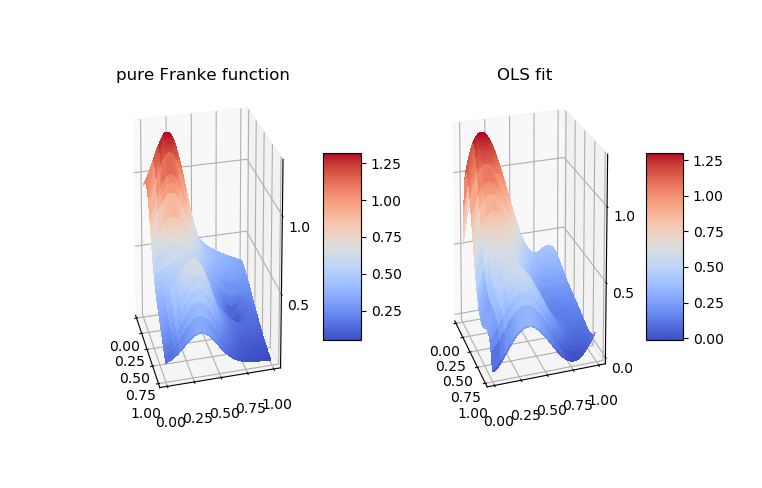
\includegraphics[scale=0.6]{frankesurface.png}
\caption{
    surface plot of the franke function(left) and the ordinary least squares fit(right), 
    without resampling. The model is trained on the entire set with the franke function 
    added stochastic noise.
    The overall structure of the surface is maintained, as well as the heights. There are 
    some sharper peaks in the Franke function surface compared to the fit, but the fit is
    faithful.
}
\label{fig:frankesurface}
\end{figure}

Figure \ref{fig:frankesurface} shows the surface plot of the franke function and the OLS fit. 
Before the fit, a stochastic noise is added to the franke function and the model then tries to
find the function underneath the noise. As the image shows, there is a good overlap of the 
franke function and the fit. This is an expected result given the existance of a continuous 
function behind the surfacem which is what regression methods try to find. 

There are still some discrepancies between the franke function and the OLS fit. In addition, the 
set we plot here is the same one we use to train the model and test it's validity. There is also 
no variation in the polynomial we try to fit the function with. It might be in a sweet spot that 
emulates the franke function, or we might have simply overfitted the model to the given data, 
and if we were to provide a set which was not within the training data, the errors would grow
markedly. It is also possible that we could enhance the fit further if we were to change the 
complexity of the model further.

The confidence interval of $\beta$ could provide some insight into the variance in the model. 
The confidence interval gives a measurement of how far out from the chosen value you would have 
to vary to be certain that a given percentage of the data was accounted for. 

\begin{figure}
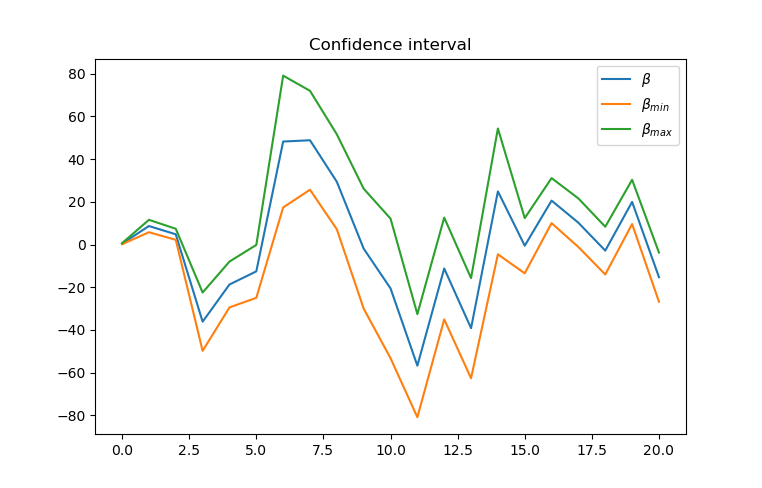
\includegraphics[scale=0.7]{frankeci.png}
\caption{
    Confidence interval of the $\beta$ values for the OLS fit sans any resampling. 
    The interval shows the range in order to include 96\% of the target values. There are 
    areas with a wider band, and the difference seems to be up to nearly 30\% of the given 
    $\beta$ value. The axis dimensions here are generally omited, as the 1. axis follows the 
    arrays without more than the index, and the 2. axis represents the coefficient values for
    the fit. These are dimensionless. 
}
\label{fig:frankeolsci}
\end{figure}

The interval is of a breadth that is not insignificant given the values of $\beta$, varying at 
times up to about 30\% of the actual beta value.

\begin{table}[H]
\centering
\begin{tabular}{ || c | c ||}
\hline
\hline
MSE & $R^2$ \\          %output: run of "initialols.py"
\hline                  %R^2 is:  0.8864615284145027
0.0118 & 0.8865 \\      %MSE is:  0.011795609124713467
\hline
\hline
\end{tabular} 
\caption{
    Mean squared error and $R^2$ function for the OLS fit of the franke function without 
    resampling. The mean squared error is fairly small, but this is not strange considering
    the fact that there is indeed a function creating the data. 
}
\label{tab:frankeolserror}
\end{table}

Calculating the mean squared error, or residual sum of squares, as seen in table 
\ref{tab:frankeolserror} reveals that the relative error of the prediction lies at about 1\%, 
and with an $R^2$ of nearly 90\% tells us that the variance seen is mostly predicted by the 
model. Though this does not rule out overfitting since the calculations have been performed on 
the same set we trained the model on. 


With the implementation of f-fold cross validation, the degree of overfitting vs. prediction can
be examined further.

\begin{figure}
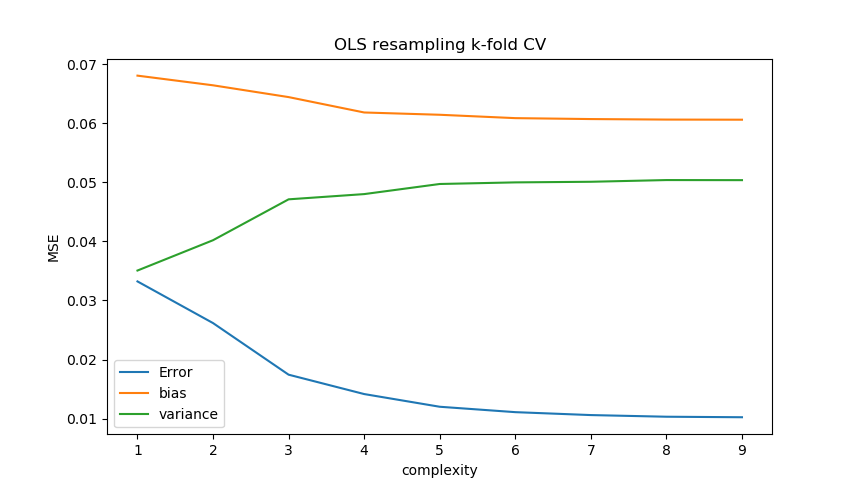
\includegraphics[scale=0.7]{frankeolsbiasvariance.png}
\label{fig:frankeolsbiasvariance}
\caption{
    OLS fit of franke function with $k=5$ folds. the complexity along the 1. axis refers
    to the polynomial degree of the fit, while the poorly named "MSE" axis depicts the 
    numerical values of bias, variance and error. These measurements are made on varying test
    sets, and as such is not a great representation of the model, but there is a definitive 
    trend for bias to fall, while variance increases with model complexity.
}
\end{figure}

As discussed above, we can see in figure \ref{fig:frankeolsbiasvariance} that the model's 
bias decreases with increasing model complexity, while the variance grows. Though this is 
hardly an ideal image, and the results being compared aren't based on a common set, but 
rather the test set at each round in the k-fold rotation. This makes the values shown, such 
as the error highly suspect. the plot does showcase the expected trends in bias and variance, 
however. And this was the main point in this stage. \\

In order to better fit a model for which there is no known function governing the outputs, 
the shrinkage methods discussed above are better suited. And the added bonus of shrinking the
output along axes not imediately along the prime axes of $\mathbf{X}$ does produce far neater 
gradient along a surface projected by the model. Implementing the Ridge regression method for 
the values and thus adding the super parameter $\lambda$ to the mix, allows us to create a 
heatmap of the error for the various $\lambda$'s and degrees of complexity.

\begin{figure}
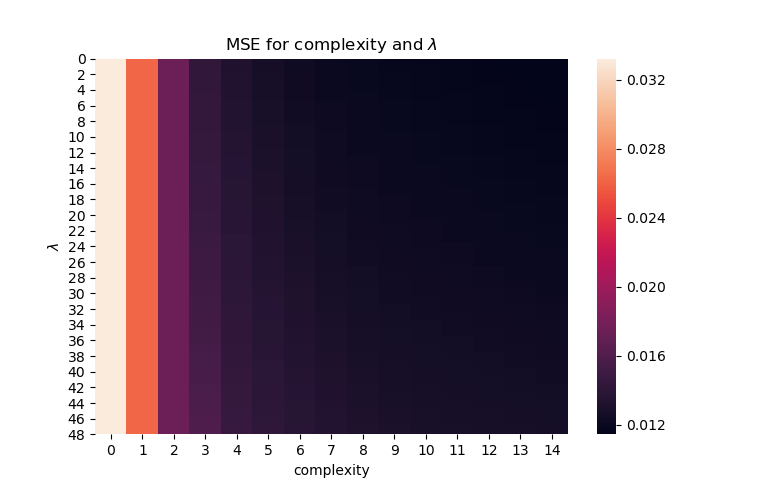
\includegraphics[scale=0.7]{frankeridgemseheatmap.png}
\label{fig:frankeridgemseheatmap}
\caption{
    Heatmap of the MSE for Ridge Regression of the franke function for various $\lambda$ and 
    degrees of complexity in the fit. The error here seems to range from 1\% to roughly 3\%, 
    with the greatest errors towards the simplest it and the lowest hyper parameter. This is 
    in accordnance with the expectation for prediction error, as the error plotted is essentially
    the training error. As we approach greater complexity, the variance also increases, as seen
    in figure \ref{fig:frankeridgevarianceheatmap}, the variance quickly explodes. 
}
\end{figure}

\begin{figure}
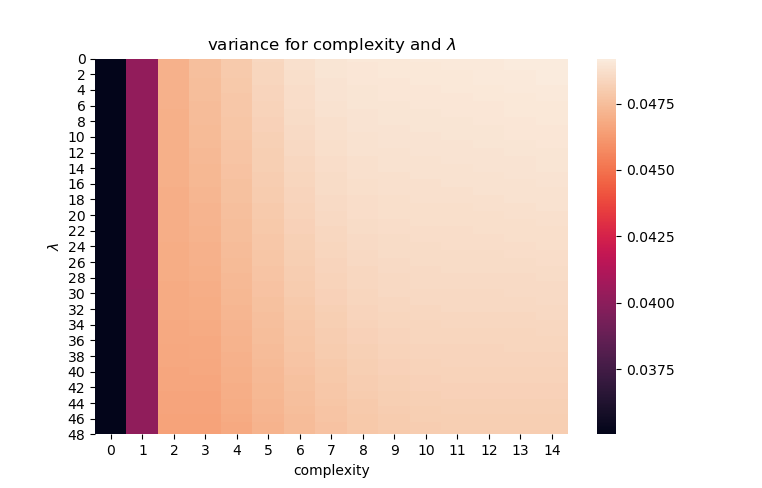
\includegraphics[scale=0.5]{frankeridgevarianceheatmap.png}
\label{fig:frankeridgevarianceheatmap}
\caption{
    Heatmap of the variance for Ridge regression of the franke function over various 
    $\lambda$ and degrees of complexity. As one would expect, the variance is least when 
    the polynomial degree of the model is low, and for the greatest shrinkage of $\lambda$, 
    though the latter has a weaker effect, as it per definition shrinks the lower variance 
    elements. 
}
\end{figure}

As we can se in figure \ref{fig:frankeridgemseheatmap}, the error falls of greatly with
increasing polynomial degree for the fit, and for lower shrinkage $\lambda$. This is not
not unexpected, given the franke function is an actual continuous function. Therefore, the
closest fit is without shrinkage. The continuous lowering of the error as we increase in
complexity speaks to the fact that the heatmap is made from the training data, and as such 
we see the downward trend of fit for the training set, and not the actual predictions of the 
functions. \\

Implementing the Lasso method for the franke function, the minimization is a lot more challenging
than with the linear case. As such, the pythno scikitlearn library was utilized for the fit and
prediction of the model here. 

\begin{figure}
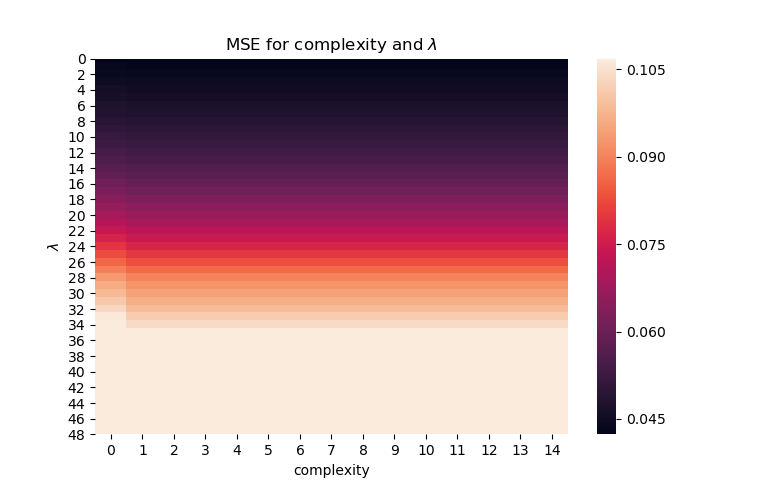
\includegraphics[scale=0.7]{frankelassomseheatmap.png}
\label{fig:frankelassomseheatmap}
\caption{
    
}
\end{figure}

\section{Conclusion}
    Conclusions and perspectives\\
    o   State main findings and interpretations \\
    o   Try as far as possible to present perspectives for future work. \\
    o   Try to discuss the pros and cons of the methods and possible improvements. \\
\section{Appendix}
    any extra material \\
    o   Additional calculations used to validate code. \\
    o   Selected calculations. Can be listed with few comments. \\
    o   Listing of code if necessary. \\
    Consider moving parts from methods to appendix. A webpage is also an appropriate place
    for a lot of this type of info. \\\\

%bibliography
 %References
    o   Always reference material you base your work on, either scientific articles/reports
        or books. \\
    o   Refer to articles as: name(s) of author(s), journal, volume(Bold), page and year in
        parenthesis. \\
    o   Refer to bookds as: name(s) of author(s), title of book, publisher, place and year, 
        eventual page numbers. \\

\end{document}
%/////////////////////

